\documentclass[conference]{IEEEtran}
\IEEEoverridecommandlockouts
% The preceding line is only needed to identify funding in the first footnote. If that is unneeded, please comment it out.
\usepackage{cite}
\usepackage{amsmath,amssymb,amsfonts}
\usepackage{algorithmic}
\usepackage{graphicx}
\usepackage{textcomp}
\usepackage{xcolor}
\def\BibTeX{{\rm B\kern-.05em{\sc i\kern-.025em b}\kern-.08em
    T\kern-.1667em\lower.7ex\hbox{E}\kern-.125emX}}
\graphicspath{{./img/}}
\begin{document}

\title{Chatbot Implementation Report\\
{\footnotesize \textsuperscript{}Chatbot: @COMP7940\_group6\_bot Github: https://github.com/hrjlhy123/comp7940-group6-project}
}

\author{\IEEEauthorblockN{Ruojie HAO, Jack}
\IEEEauthorblockA{\textit{Hong Kong Baptist University}\\
Hong Kong\\
21415315@life.hkbu.edu.hk}
\and
\IEEEauthorblockN{Zimeng ZHAO}
\IEEEauthorblockA{\textit{Hong Kong Baptist University}\\
Hong Kong\\
21458839@life.hkbu.edu.hk}
\and
\IEEEauthorblockN{Khem LIMBU}
\IEEEauthorblockA{\textit{Hong Kong Baptist University}\\
Hong Kong\\
21470634@life.hkbu.edu.hk}
}

\maketitle

\begin{abstract}
This is the project report for group 6 of COMP7940 Cloud Computing. The purpose of this report is to explain the different components of the chatbot (@COMP7940\_group6\_bot). The project is hosted at: https://github.com/hrjlhy123/comp7940-group6-project
\end{abstract}

\begin{IEEEkeywords}
Chatbot, DigitalOcean, Server, Database
\end{IEEEkeywords}

\section{Introduction}
The project can be divided into 3 main parts - the cloud platform on which the application is hosted by DigitalOcean, a MySQL database hosted on DigitalOcean, and the front-end graphical user interface of the chatbot which is in Telegram. This document is instructed by \LaTeX. 

\section{Architecture}
\begin{figure}[h]
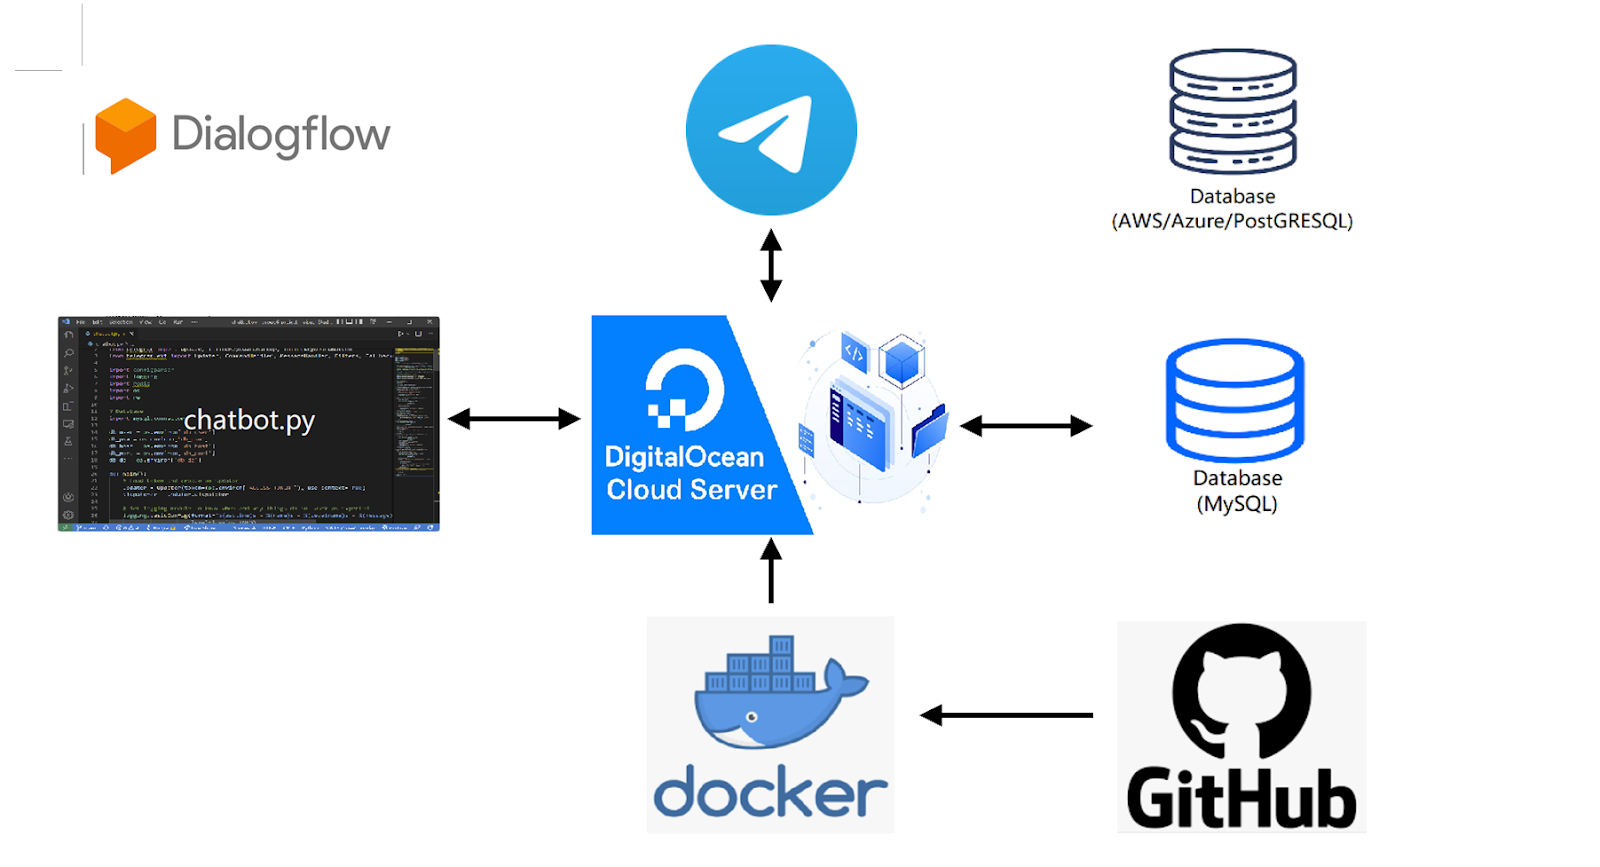
\includegraphics[scale=0.18]{1} 
\caption{Chatbot System Architecture}
\end{figure}
The architecture of the chatbot can be summarized as follows: The chatbot is hosted on DigitalOcean's server called APP, and the database is hosted at DigitalOcean's Singapore Data Service Center. The server and database are proxied separately, and we do not use a PostgreSQL proxy database under the same server for hosting. Telegram is used as the user interface to realize certain functionalities of the chatbot application. Moreover, we also used the docker hub and the container method for efficient version control and deployment of the application. Lastly, the source code has been uploaded to Github and team members can do version control from there.
We tried some more advanced services such as Google Dialogflow, an AI language-recognition chatbot, or Microsoft's Azure database and Amazon's AWS database.
\section{Applications}
\subsection{Application of server}
DigitalOcean (DO) is an infrastructure-as-a-service (IaaS) service where DO provides users with the basic infrastructure and users can decide on the different types of OS and configurations. That being said, the chatbot application is hosted on DigitalOcean Server and it can be started or stopped using the console found on the website. 
\begin{figure}[h]
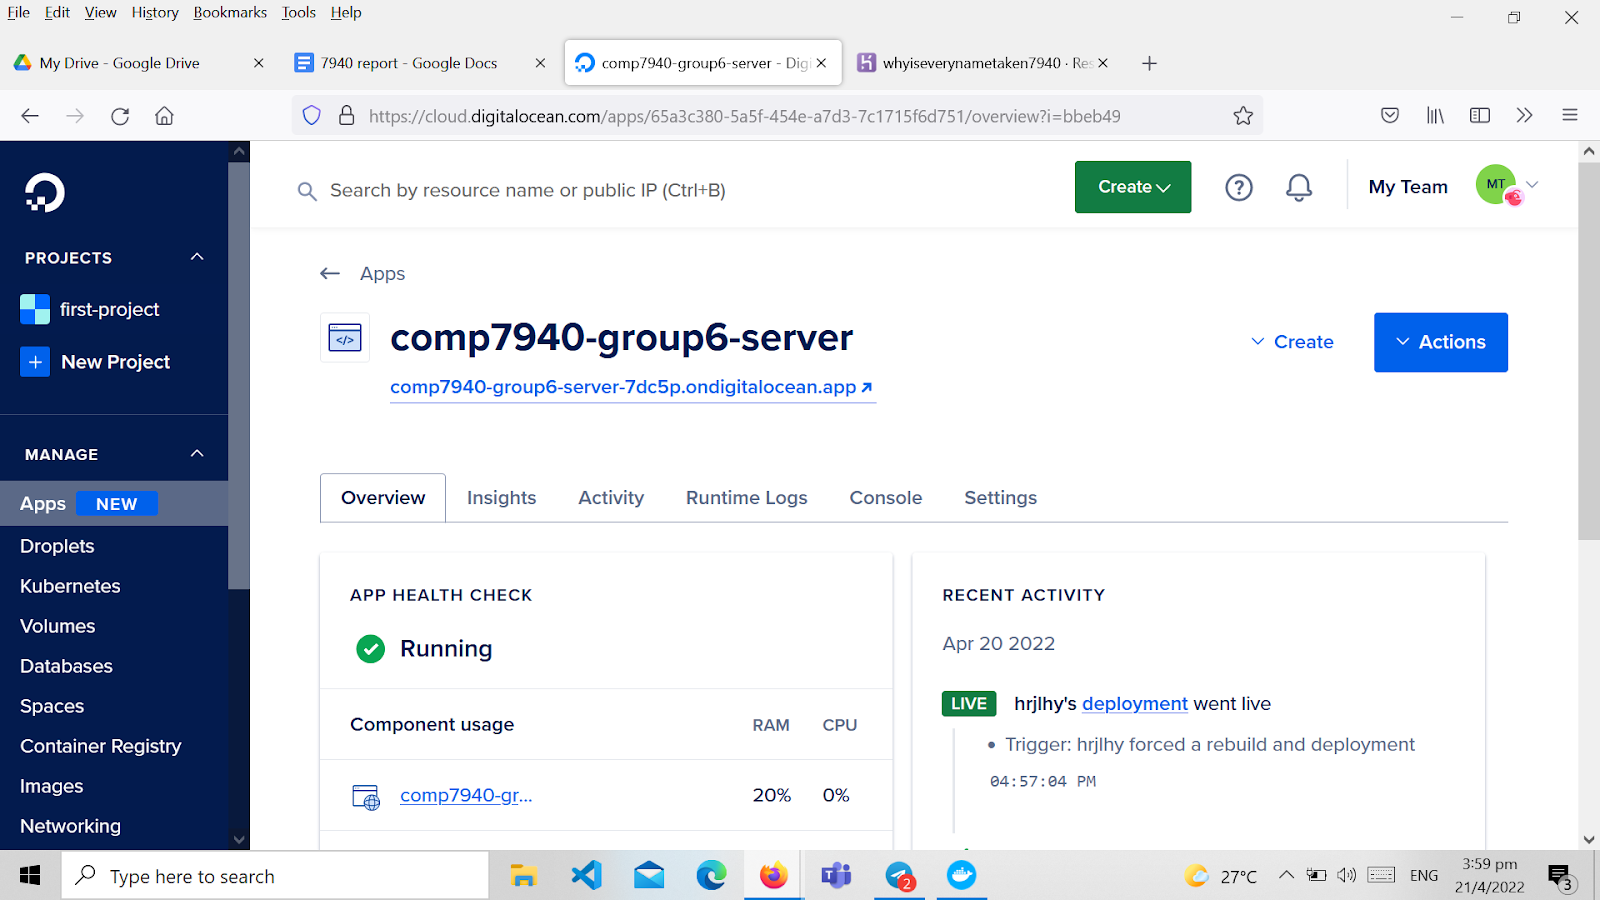
\includegraphics[scale=0.155]{2} 
\caption{Chatbot application running via DigitalOcean}
\end{figure}

\subsection{Application of database}
\subsubsection*{DigitalOcean Database}
The database of choice was MySQL. We used it to create simple tables for the chatbot to retrieve information and reply back to users. Moreover, we used Tableau to connect with database and manage it.
\begin{figure}[h]
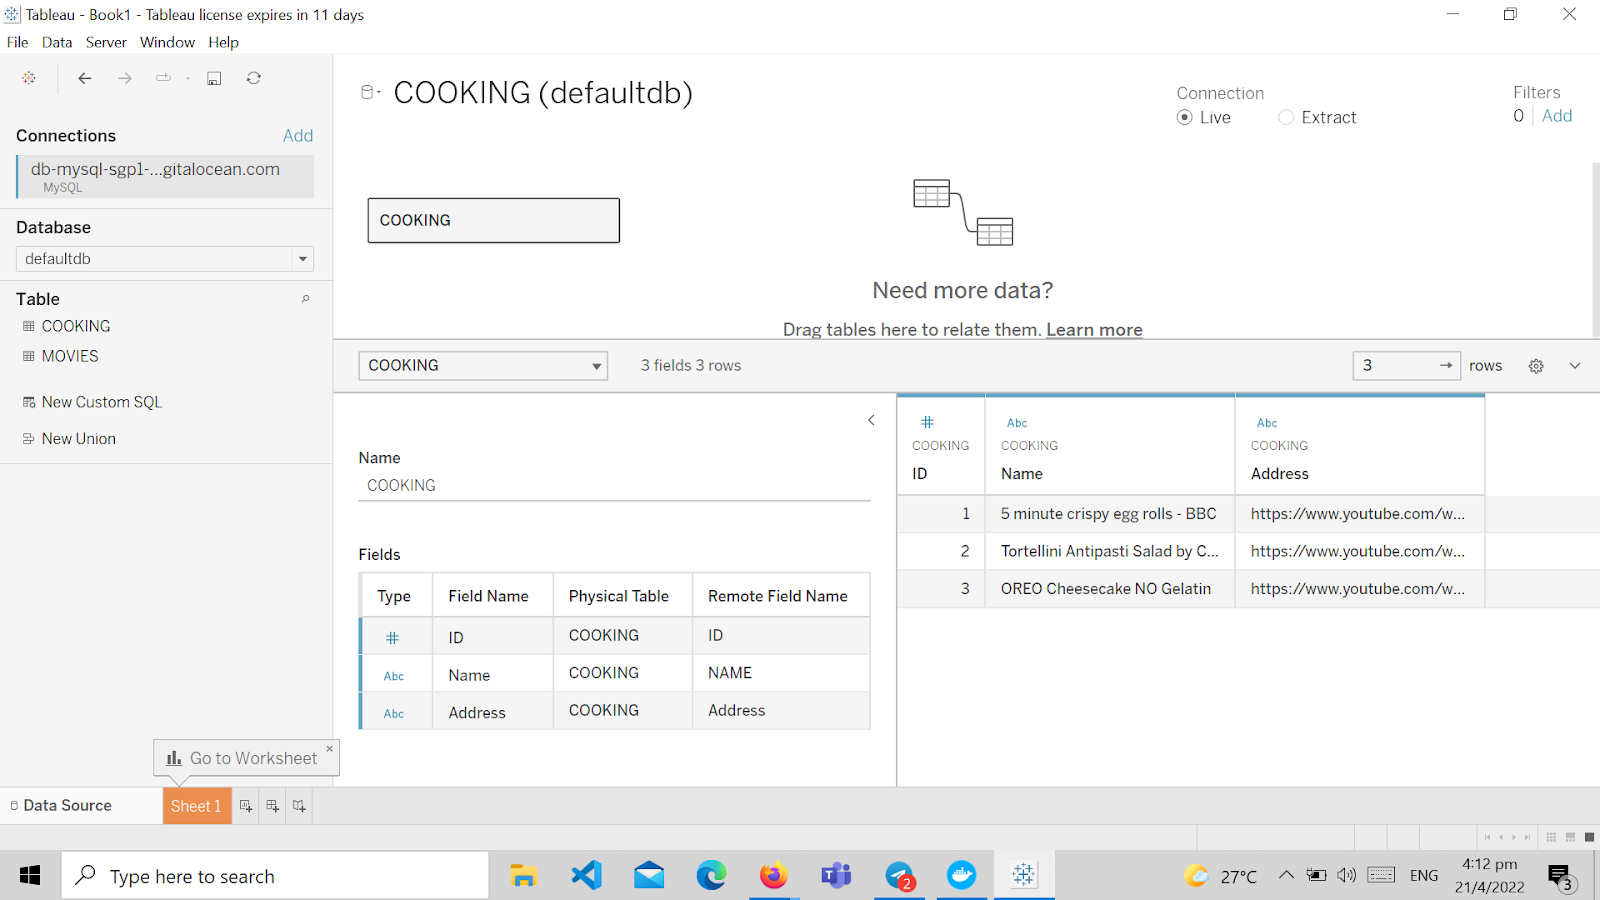
\includegraphics[scale=0.155]{6} 
\caption{Examples of our database tables}
\end{figure}
\subsubsection*{Experimenting with other Database}
We tried some other databases like AWS database, Azure database, and PostgreSQL database which are very advanced and efficient, but they are not very "cloudy", so we finally decided to abandon them and choose the more suitable DigitalOcean database.
\subsection{Application of chatbot}
\subsubsection*{chatbot.py}
Our application started up by running “python chatbot.py”. The main concept of the project was to design a practical chatbot that would be able to respond with useful information from database to users who could then share the information with other users.

Our chatbot is not only capable of repeating basic greetings, but can also recommend Movies, TV shows, or cooking videos to the user based on their input. As a result, the user is able to get content catered to their tastes and can also recommend said content to other users. This way, users of our platform can learn new things related to their interests and also interact with other users safely in these trying times.
\begin{figure}[h]
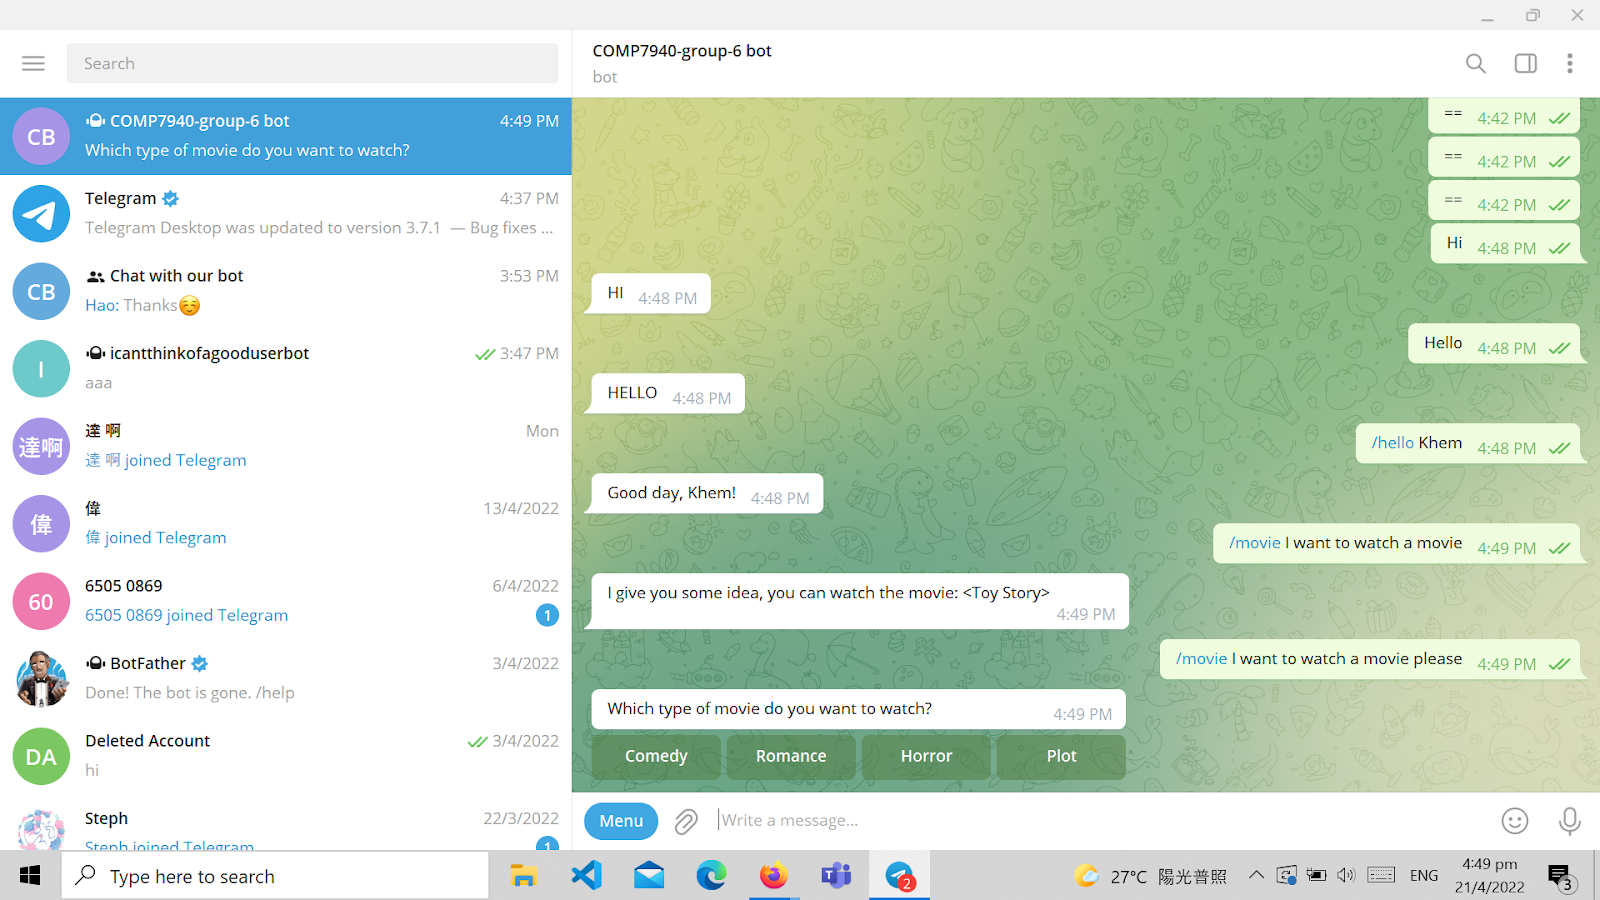
\includegraphics[scale=0.155]{8} 
\caption{Greetings and movie recommendation function}
\end{figure}

The chatbot is able to give different recommendations depending on the user’s input, i.e. movie genre, type of food, etc. Moreover, the movie\_add function allows users to also add movies to the database which has 10GB of space. Besides that, the links for the cookery videos can also be shared between users. Ultimately, the long-term goal would be to create a sense of community among users who have similar interests, i.e. watching movies, and cooking, and allow them to share their opinions in a safe manner.

\subsubsection*{Experimenting with AI chatbot (Google Dialogflow)}
Google Dialogflow is a natural language understanding platform that makes it easy to design and integrate conversational user interfaces into mobile applications, web applications, devices, bots, interactive voice response systems, and more. We performed a Google Dialogflow deployment and executed it in our chatbot platform successfully.

\section{Project management approach}
\subsection*{Before building up the method}
We tried to use the public repository of the docker hub to manage the chatbots on the server. At first, we did not build the push workflow mentioned in the latter part. We took the “docker commit” and “docker push” commands to upload the files to the docker hub, after which we manually deploy them on the server.
\subsection*{Github push and Docker build}
\begin{figure}[h]
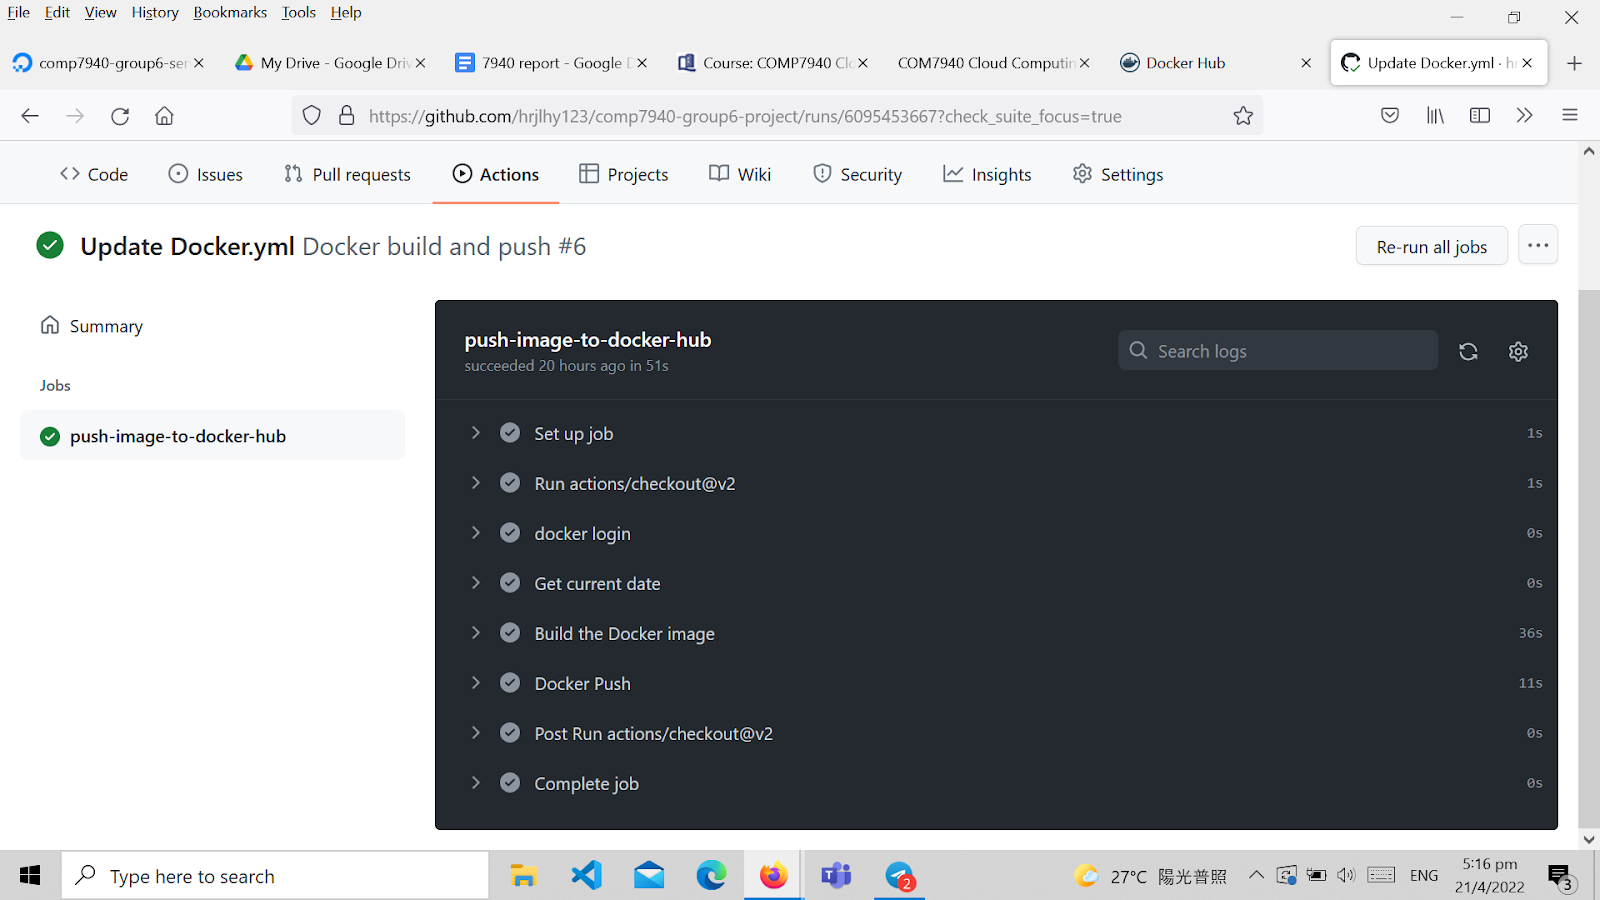
\includegraphics[scale=0.155]{13} 
\caption{Workflow - Github-push-and-Docker-build}
\end{figure}
As seen from the GitHub repo, this project contains various files and folders. Moreover, there are many dependencies that need to be run in order to execute the application. Therefore, the docker container technique has been in order to save time and effort.
Docker and Dockerhub by extension is a form of platform-as-a-service (PasS). It uses OS-level virtualization to package applications in containers. This allows for quick startup of applications and also efficient version control. Besides that, we have used GitHub workflows and integrated the Github-push-and-Docker-build workflow. By integrating this workflow, the container will be automatically updated and pushed every time GitHub experiences a new push.
\subsection*{Python security check}
A python security check has also been integrated into the workflow. This security check taps into the SafetyDB database and continuously checks for known python security vulnerabilities. Therefore, reinforcing the security aspect of the application.

\begin{thebibliography}{00}
\bibitem{b1} “Dialogflow documentation  |  google cloud,” Google. [Online]. Available: https://cloud.google.com/dialogflow/docs. [Accessed: 21-Apr-2022]. 
\bibitem{b2} “Difference between IAAS, paas and SAAS,” GeeksforGeeks, 16-Jun-2020. [Online]. Available: https://www.geeksforgeeks.org/difference-between-iaas-paas-and-saas/. [Accessed: 21-Apr-2022]. 
\bibitem{b3} S. Usher, “Build Modern Applications with Free Databases on AWS,” Amazon, 2021. [Online]. Available: https://aws.amazon.com/free/database/. [Accessed: 21-Apr-2022]. 
\end{thebibliography}

\subsection{Appendix: Screenshots}
\begin{figure}[h]
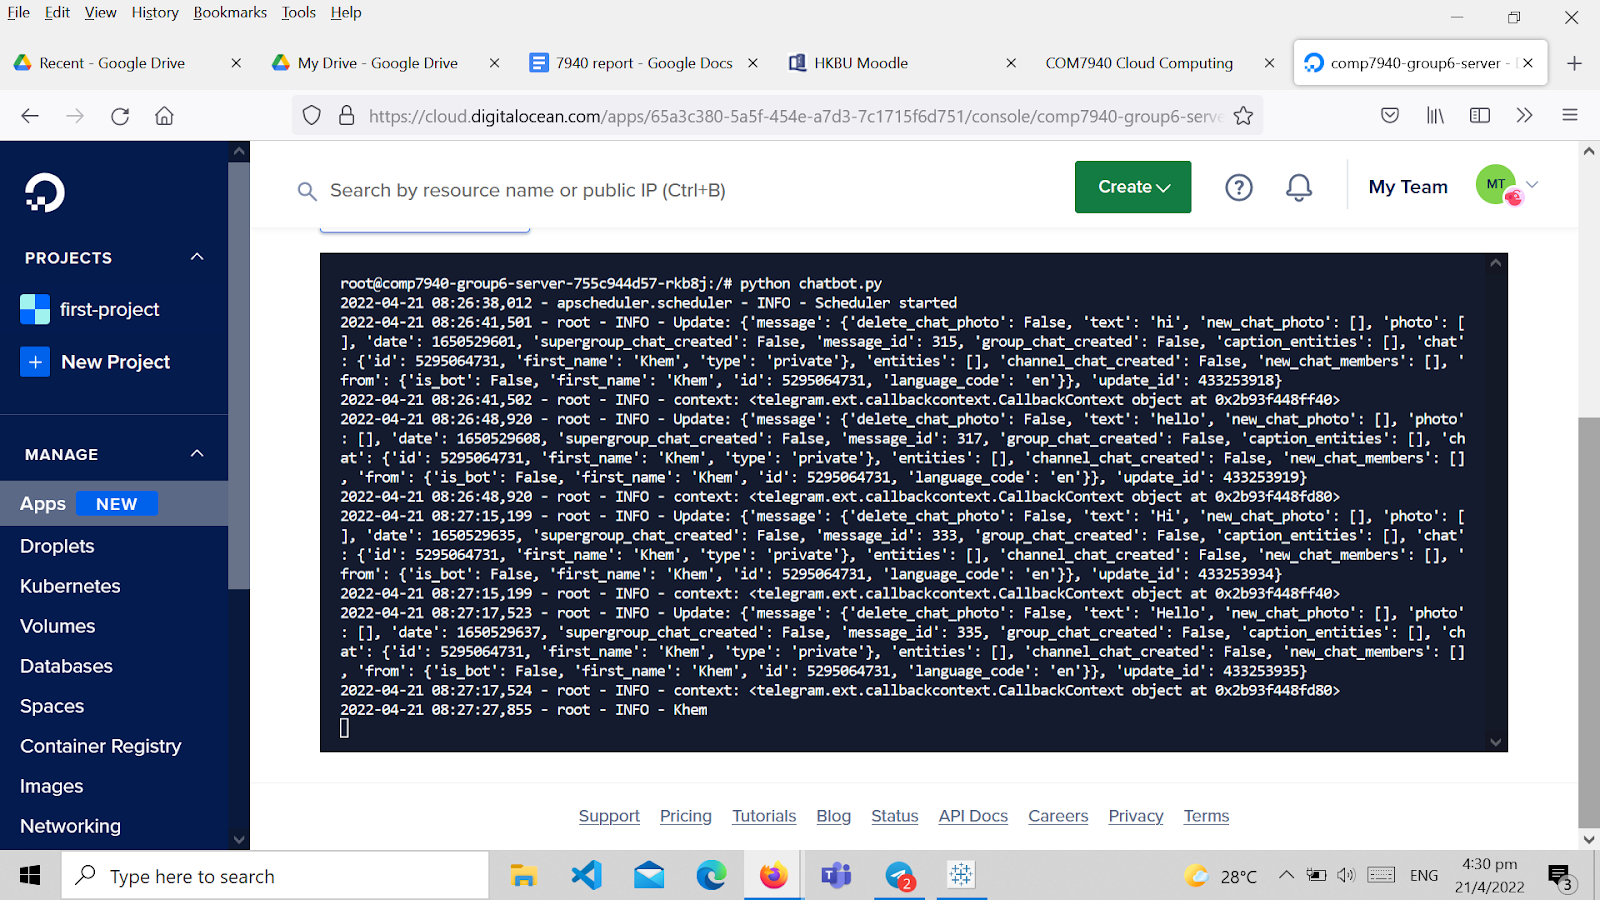
\includegraphics[scale=0.155]{3} 
\caption{Console and application log}
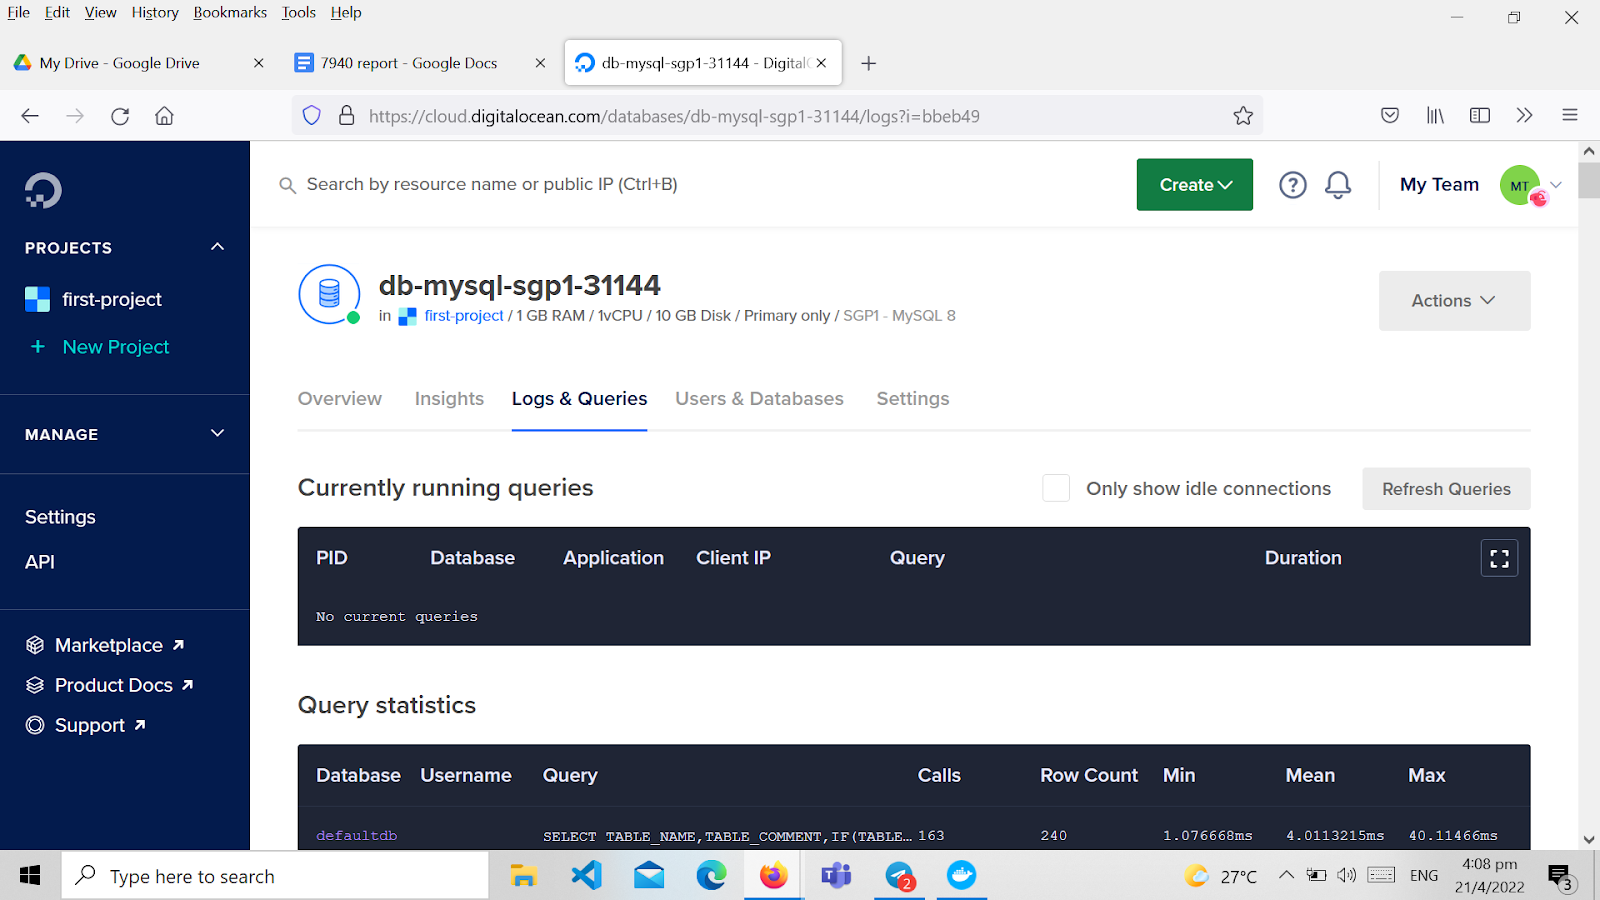
\includegraphics[scale=0.155]{4} 
\caption{MySQL database hosted on DigitalOcean}
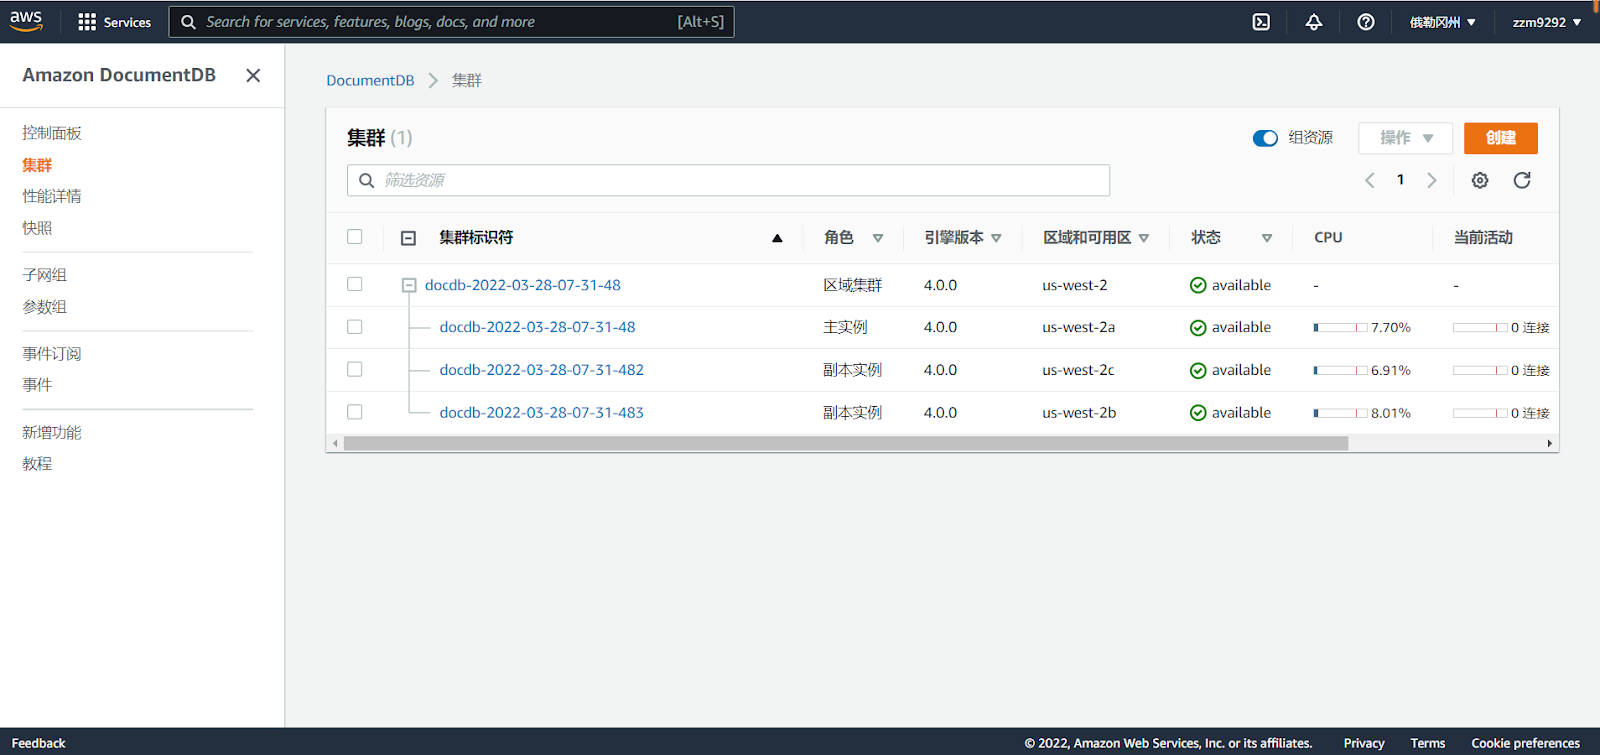
\includegraphics[scale=0.155]{7} 
\caption{The AWS database that we abandoned}
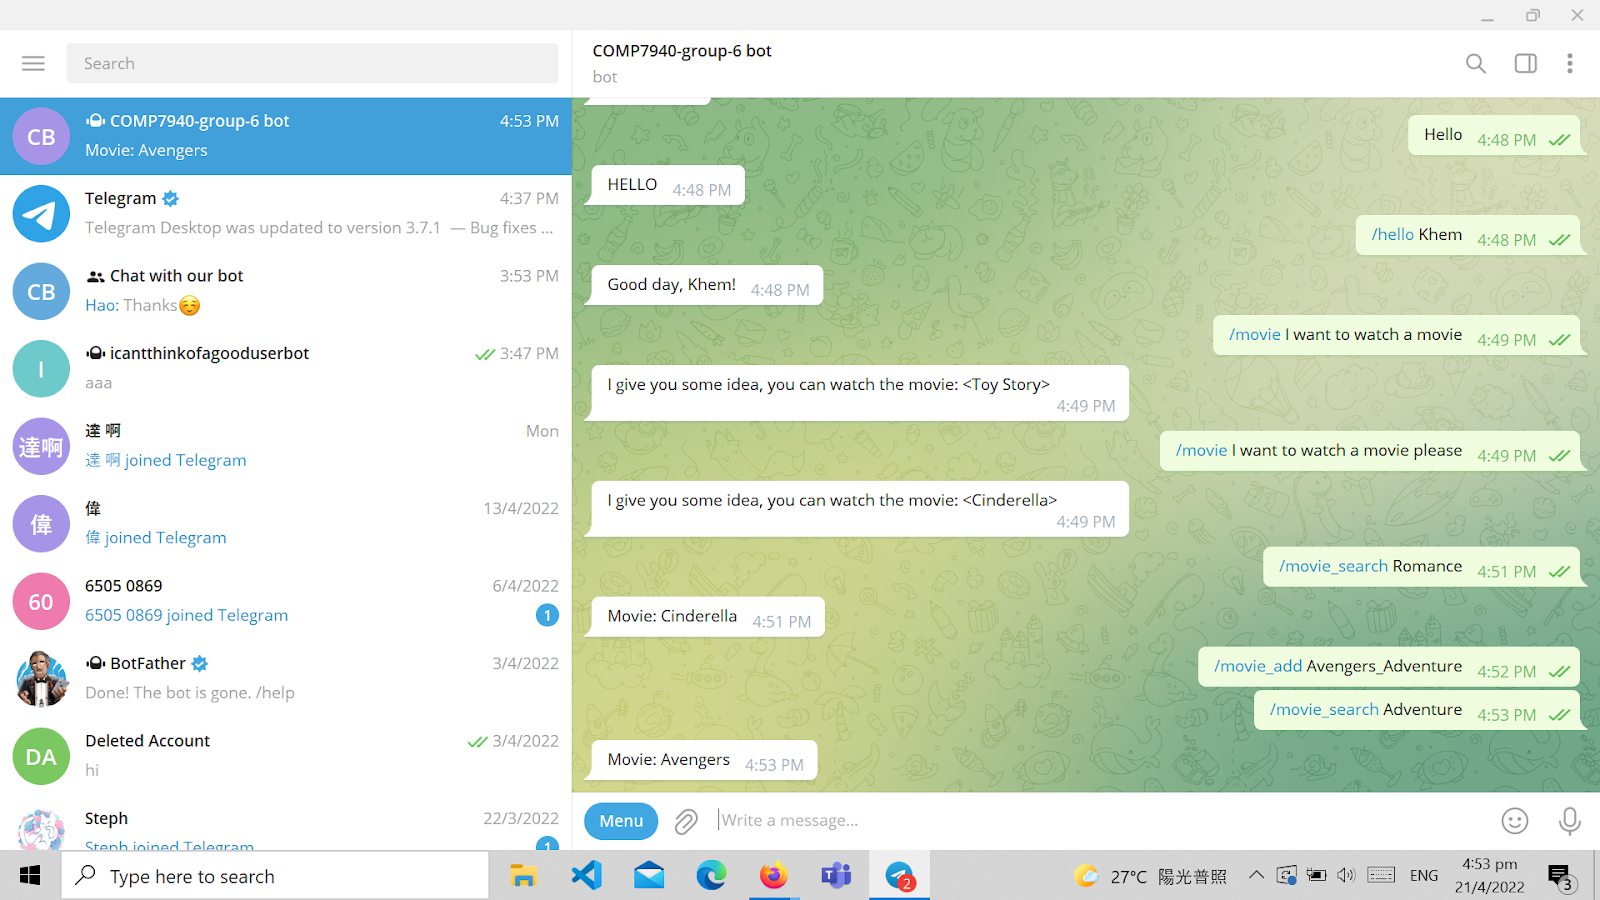
\includegraphics[scale=0.155]{9} 
\caption{Movie add (name\_genre) and search function}
\end{figure}
\begin{figure}[h]
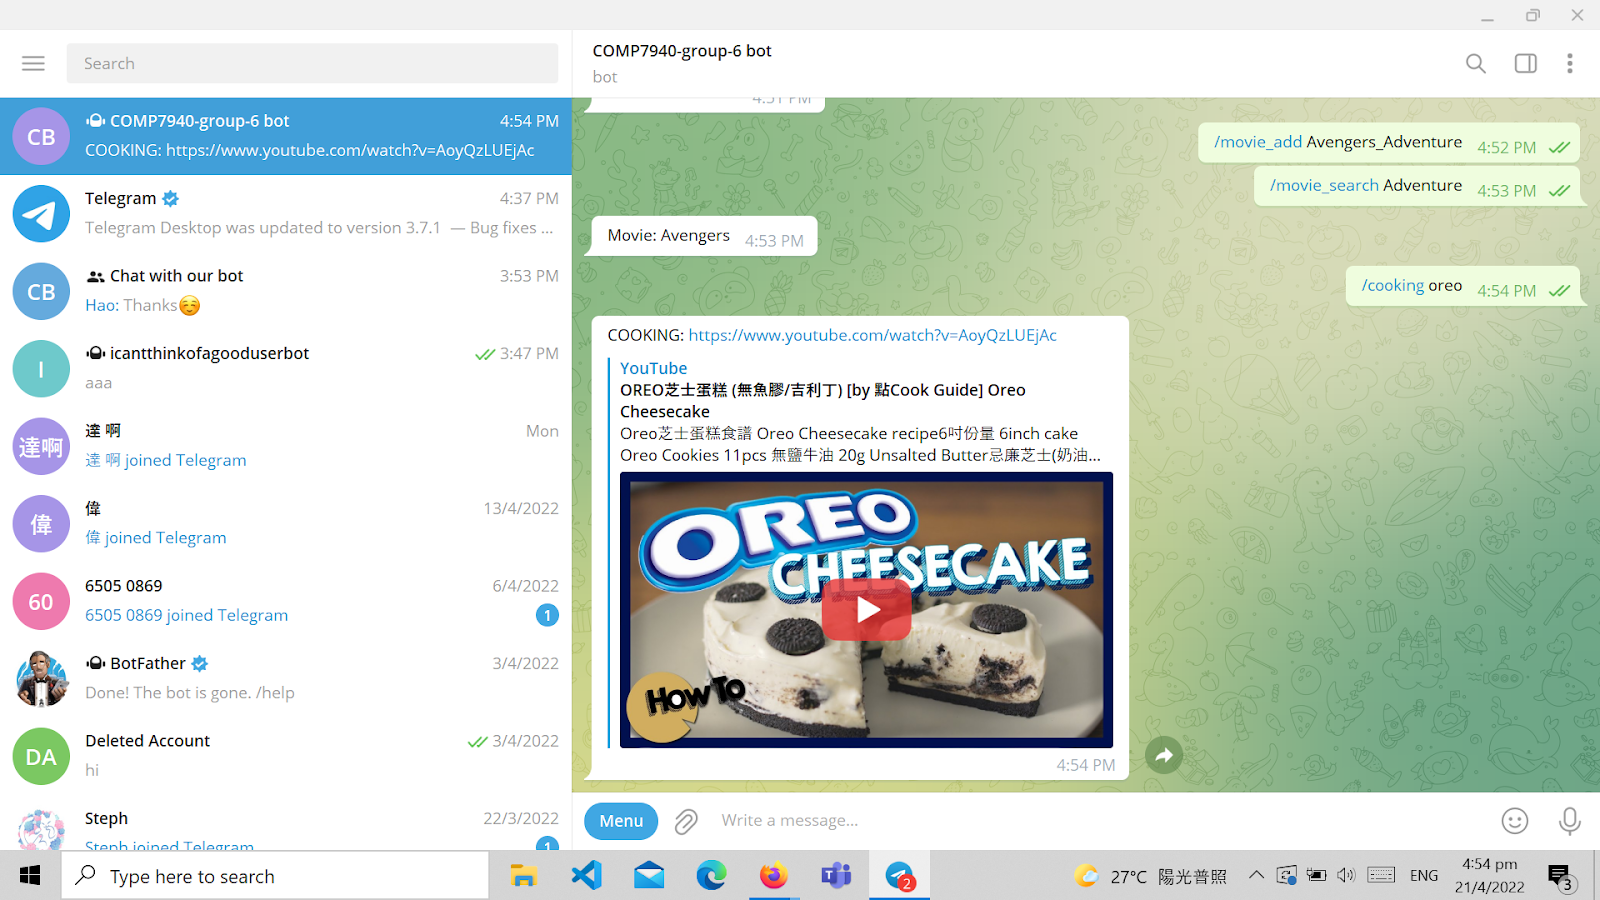
\includegraphics[scale=0.155]{10} 
\caption{Cookery video recommendation}
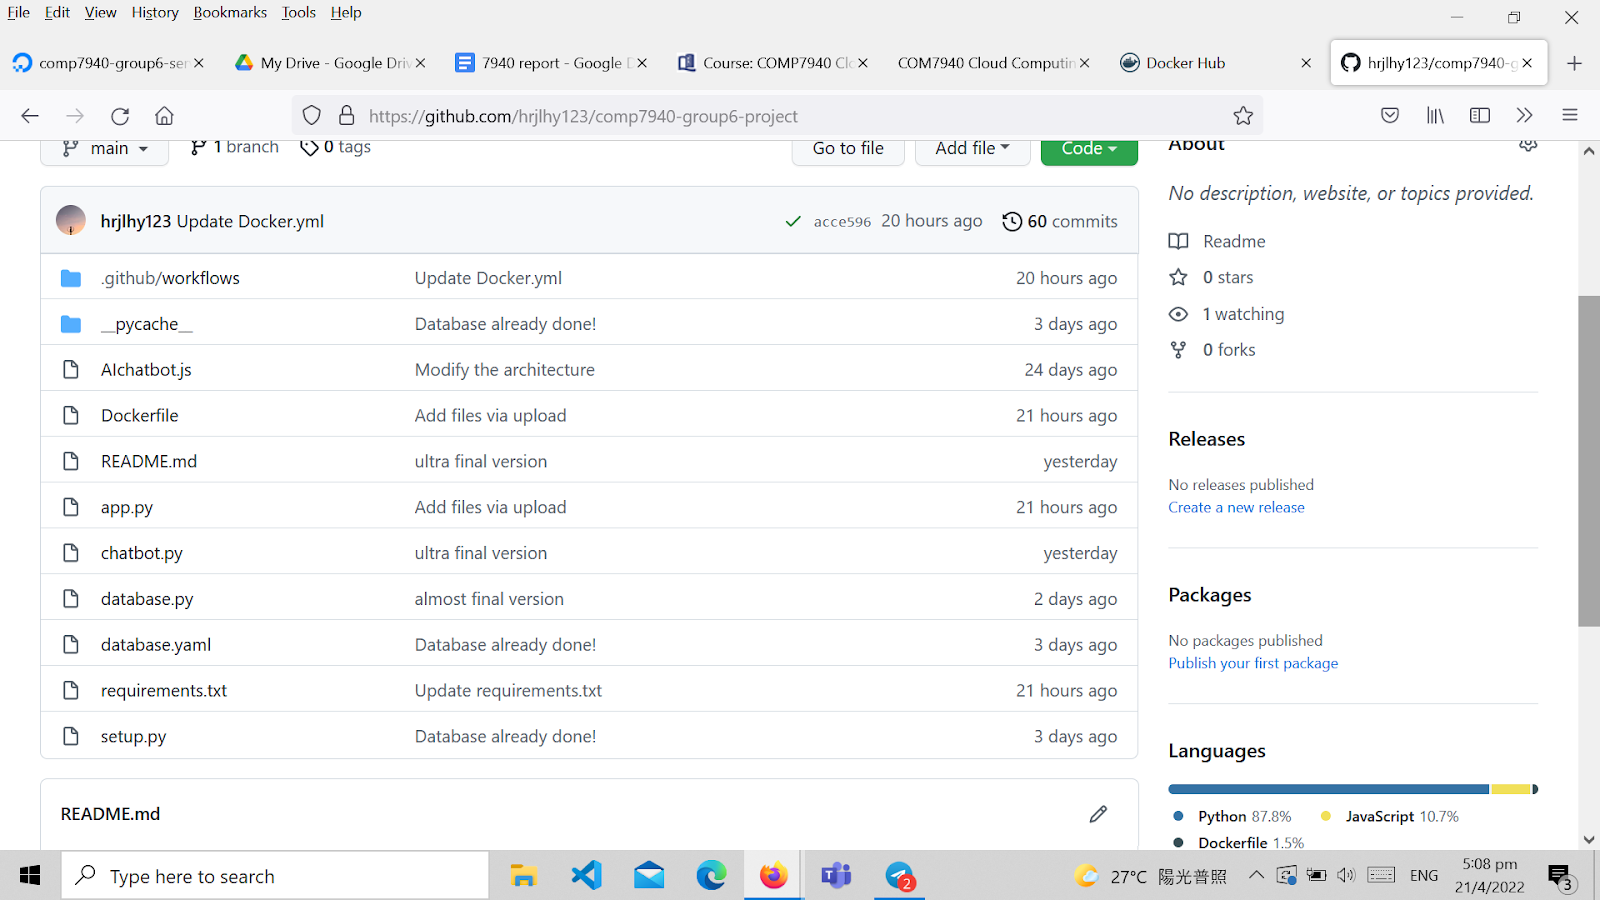
\includegraphics[scale=0.155]{11} 
\caption{Overview of files and folders}
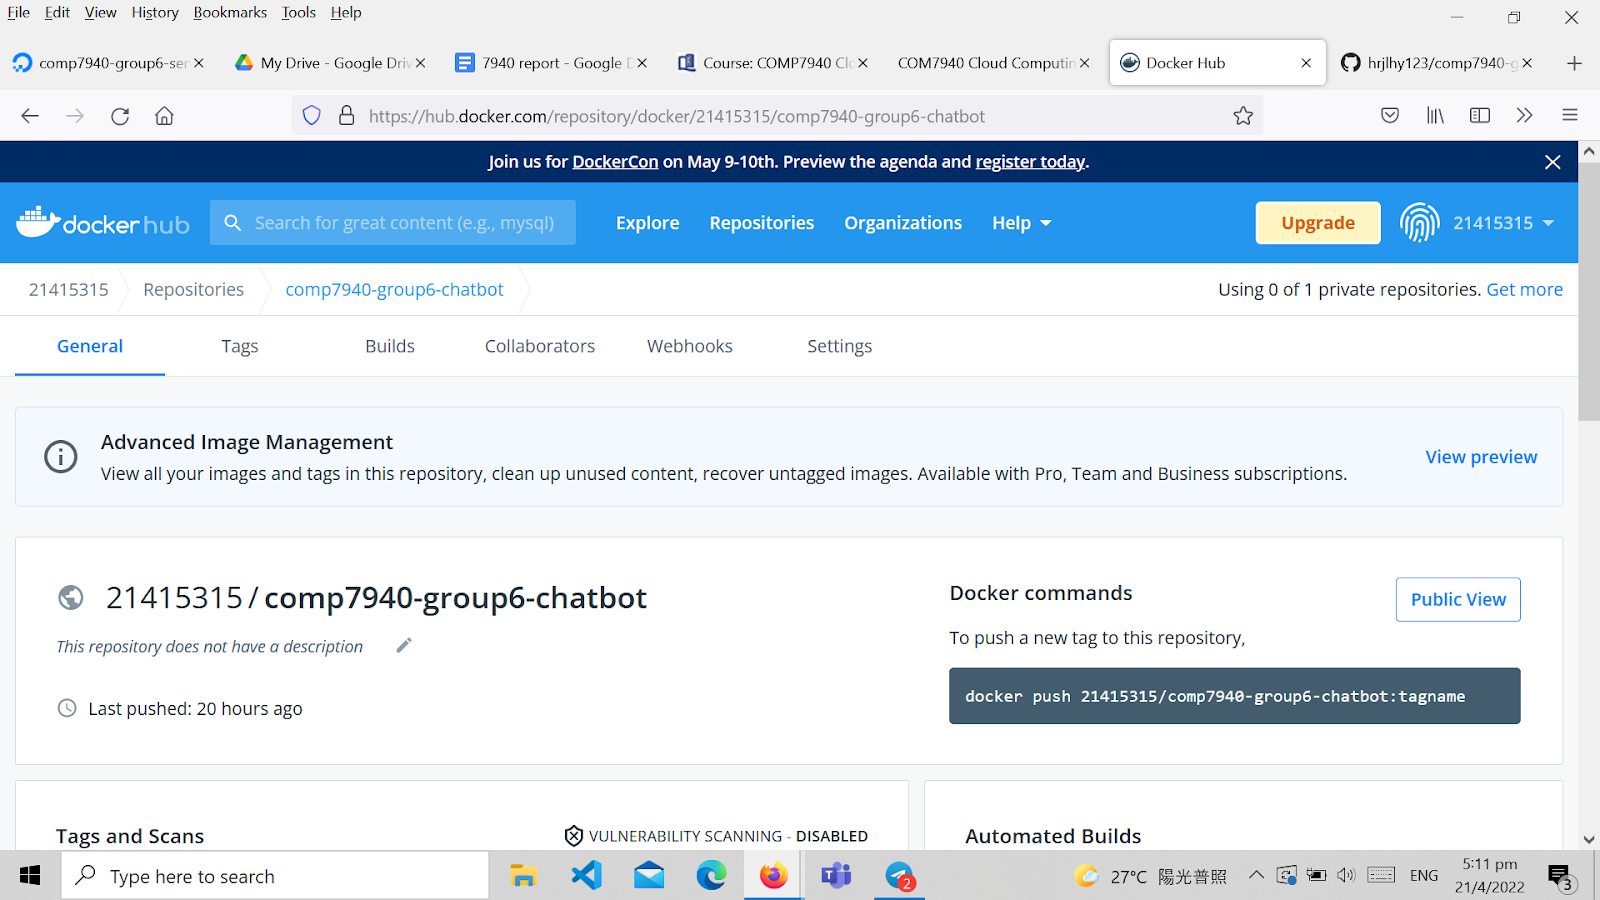
\includegraphics[scale=0.155]{12} 
\caption{Docker image}
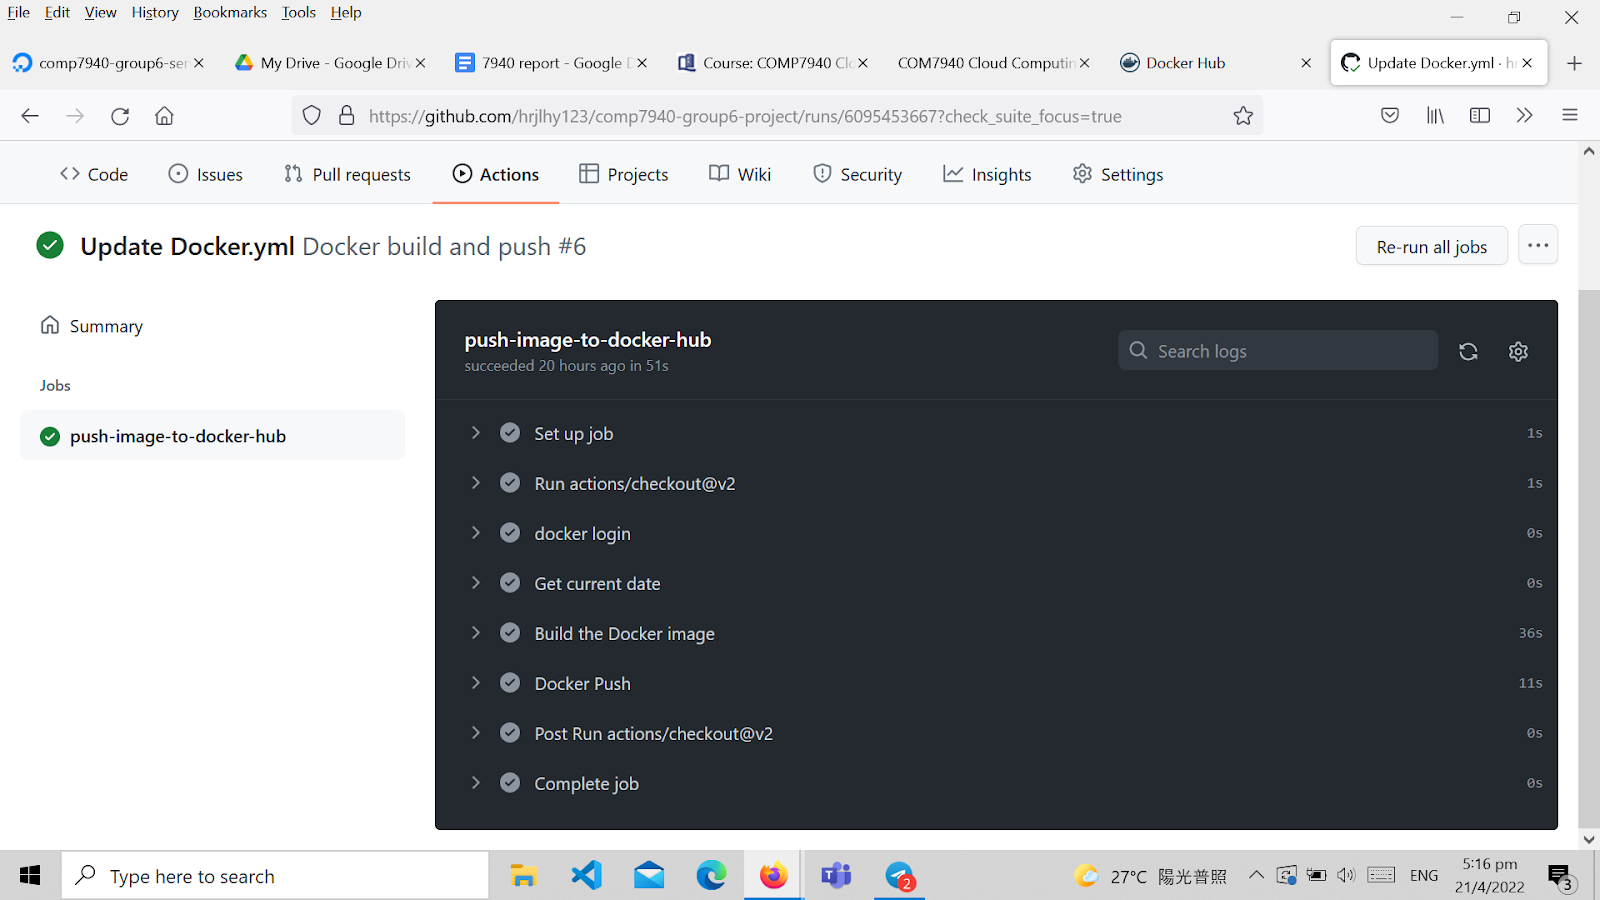
\includegraphics[scale=0.155]{13} 
\caption{Workflow - Python safety check}
\end{figure}
\vspace{12pt}
\color{red}
\end{document}
